We propose the algorithm latent ranker algorithm, abbreviated as LRA (see Algorithm \ref{alg:latent-rank}) for solving the personalized ranking problem. This algorithm is motivated by the ranked bandit algorithm (RBA) from \citet{radlinski2008learning}. The RBA is suited for finding a global ranking of items amongst all the users without being personalized for individual user and so it will fail to suggest the best ranking for each user sorted by their preference from high to low. LRA is divided into two main components, the $d$ column MABs denoted by MAB$_1(n)$, MAB$_2(n), \dots,$ MAB$_d(n)$ and the $K$ row weighted majority algorithms (WMA) for each user $[K]$. The WMA from \citet{littlestone1994weighted} is suited for the total information setting. Note, that in our setting all the clicks by the user is seen by the system and so it is a total information setting. Each WMA consist of $d!$ arms for each of the permutations of rank $d$. Its goal is to suggest a permutation $\pi_{i_t}(J_t)$ such that the best item for the user $i_t$ is in rank $1$ of the permutation $\pi_{i_t}(J_t)$.  

%\todoan{complete feedback?} \todosb{kept as total info} 
%is motivated \todoan{is it just motivated or has this algorithm appeared before?}

LRA proceeds as follows. At every timestep $t\in[n],$ a user $i_t$ is revealed by nature, then the $d$ column MABs suggests columns $J_t = \lbrace {\ell}_{1}, {\ell}_{2},\dots, {\ell}_{d} \rbrace$ which it deems to be the $d$ best columns and by virtue of our setting, the $d$ hott-topics. If, there is any overlap in the suggestion, an arbitrary column is suggested which has not been selected before. Then, the row WMA for the $i_t$-th user selects a permutation $\Pi_{i_t}(J_t)$ by sampling through its distribution over the $d!$ arms and suggests a permutation $\pi_{i_t}(J_t) = \lbrace \tilde{\ell}_{1}, \tilde{\ell}_{2},\dots, \tilde{\ell}_{d}\rbrace$ such that the item in rank $1$ is the best item for the $i_t$-th user with a high probability. Note, that we leave the implementation of the column MAB to the user which can be any stochastic or adversarial base-bandit algorithm discussed in Section \ref{related}. 


%\todoan{Might have re-write the row algorithm based on Brano's new algorithm.}
%\todosb{He is asking to keep things same, have to ask again}

%\todoan{this doesn't make sense to me, global ranking for users?} \todosb{Changed, global ranking of items for all users without personalization}

Finally, after all the user clicks are recorded by the system both the column MABs and row WMA$_{i_t}(n)$ is updated. The $k$-th column MAB$_k(n)$ is updated with feedback $f_{k,t} = \max_{j\in [k]} r_t(i_t, \ell_{j,t}) - \max_{j\in [k-1]} r_t(i_t,\ell_{j,t})$. The intuition behind this update is that first the rank of the $k$-th column will be fixed and then based on that the rank of the $(k-1)$-th column will be determined.  This type of update follows from the fact that the $\max$ function is monotonic and submodular (see  section \ref{related}) and by updating $f_{k,t}$ like this the column MABs are guaranteed to find the $d$ best columns with high probability. Note that RBA is also a special case of submodular bandits such that $f_{k,t}\in\lbrace 0, 1\rbrace$ \citep{streeter2009online}. 

\begin{figure}
    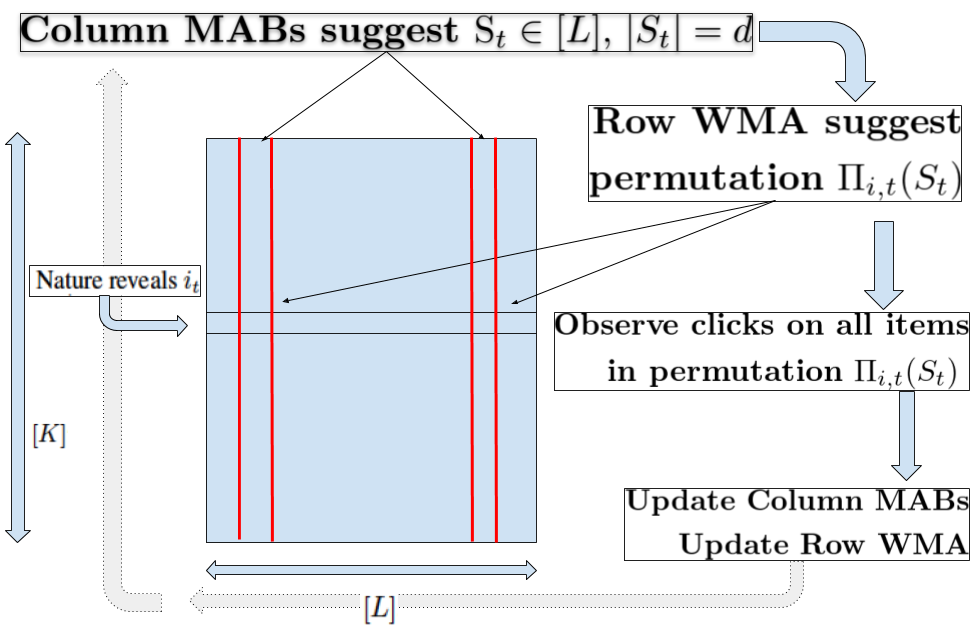
\includegraphics[scale=0.2]{img/RankedBand.png}
    \caption{Latent Ranked Bandit in rank $d=2$ scenario.}
    \label{fig:rankedbandit}
    \vspace*{-1em}
\end{figure}

The row WMA$_{i_t}(n)$ update for the $i_t$-th user is quite straightforward as all the $d$ clicks are observed (total information). Hence, LRA can easily calculate the feedback for all the $d!$ permutation of $\pi_{i_t}(J_t)$ and update its $d!$ arms representing each of those permutations. LRA calculates a weighted sum of feedback for each of the $d!$ permutation of $\pi_{i_t}(J_t)$ and update the weights and its probabilities of the corresponding permutation. An illustrative diagram of the entire process is shown in Figure \ref{fig:rankedbandit}.

%Since, we observe all the clicks by user $i_t$ (total information),


\begin{algorithm}
\caption{Latent Ranker Algorithm}
\label{alg:latent-rank}
  \begin{algorithmic}[1]
  \State \textbf{Input:} Rank $d$, horizon $n$.
  \State Initialize MAB$_1(n)$, MAB$_2(n), \dots,$ MAB$_d(n)$
  \State Initialize WMA$_1(n)$, WMA$_2(n), \dots,$ WMA$_K(n)$
    \For{$t = 1, \dots, n$}
      \State User $i_t$ comes to the system
      \For{$k = 1, \dots, d$}
      %\State // Choose $d$ items from $d$ column MABs
      \State ${\ell}_{k,t} \leftarrow$ suggest item $MAB_k(n)$
      \If{${\ell}_{k,t} \in \ell_{1, t},\dots,\ell_{k-1, t}$}
      \State ${\ell}_{k,t} \leftarrow$ Select arbitrary unselected item from $[L]\setminus \ell_{1, t},\dots,\ell_{k-1, t}$
      %\Else
      %\State $\ell_{k,t} \leftarrow \hat{\ell}_{k,t}$
      \EndIf
      \EndFor
      \State $\tilde{\ell}_{1,t},\tilde{\ell}_{2,t},\dots,\tilde{\ell}_{d,t}\leftarrow$ Permutation by WMA$_{i_t}(\ell_{1,t},\ell_{2,t},\dots,\ell_{d,t})$ by sampling  according to $p_{i_t,1},p_{i_t,2},\dots,p_{i_t,d!}$.
      %by sorting descendingly according to $w_{i_t,1},w_{i_t,2},\dots,w_{i_t,d}$.
      \State Present $\tilde{\ell}_{1,t},\tilde{\ell}_{2,t},\dots,\tilde{\ell}_{d,t}$ to user $i_t$ and record feedback $r_{t}(\tilde{\ell}_{1,t}), r_{t}(\tilde{\ell}_{2,t}),\dots,r_{t}(\tilde{\ell}_{d,t})$.
      \State Call Procedure UpdateColumnMAB
      \State Call Procedure UpdateRowWMA($i_t$)
    \EndFor
    \Procedure{UpdateColumnMAB}{}
    \For{$k = 1, \dots, d$}
    \State Update MAB$_k(n)$ with feedback $f_{k,t} = \max_{j\in [k]} r_t(i_t, \ell_{j,t}) - \max_{j\in [k-1]} r_t(i_t,\ell_{j,t})$
    % where $J_t[1: k] = \lbrace r_{t}({\ell}_{1,t}), r_{t}({\ell}_{2,t}),\dots,r_{t}({\ell}_{k,t})\rbrace$
    \EndFor
\EndProcedure
\Procedure{UpdateRowWMA}{$i_t$}
	\For{$k=1,2,\dots,d!$}
	\State $r_k = 0$ \Comment{Calculate weighted sum of rewards}
    \For{$j = 1, \dots, d$}
    \State $r_{k} = r_{k} + \frac{1}{j}r_{t}(\tilde{\ell}_{j,t})$
    \EndFor
    \State $w_{i_t,k} = w_{i_t,k} + r_k$  \Comment{Update weights}
    \EndFor
	\For{$k = 1, \dots, d!$}
	\State $p_{i_t,k} = \dfrac{\exp(w_{i_t,k})}{\sum_{b=1}^{d!} \exp(w_{i_t,b})} $ %\Comment{Update probabilities}
	\EndFor
\EndProcedure
  \end{algorithmic}
\end{algorithm}